\documentclass[]{elsarticle} %review=doublespace preprint=single 5p=2 column
%%% Begin My package additions %%%%%%%%%%%%%%%%%%%
\usepackage[hyphens]{url}
\usepackage{lineno} % add
\providecommand{\tightlist}{%
  \setlength{\itemsep}{0pt}\setlength{\parskip}{0pt}}

\bibliographystyle{elsarticle-harv}
\biboptions{sort&compress} % For natbib
\usepackage{graphicx}
\usepackage{array}
\usepackage{booktabs} % book-quality tables
\usepackage[font=small]{caption}
\usepackage[labelformat = empty,position=top]{subcaption}
\usepackage[export]{adjustbox}

%% Redefines the elsarticle footer
%\makeatletter
%\def\ps@pprintTitle{%
% \let\@oddhead\@empty
% \let\@evenhead\@empty
% \def\@oddfoot{\it \hfill\today}%
% \let\@evenfoot\@oddfoot}
%\makeatother

\newcommand{\subfigimg}[3][,]{%
	\setbox1=\hbox{\includegraphics[#1]{#3}}% Store image in box
	\leavevmode\rlap{\usebox1}% Print image
	\rlap{\hspace*{10pt}\raisebox{\dimexpr\ht1-2\baselineskip}{#2}}% Print label
	\phantom{\usebox1}% Insert appropriate spcing
}

% A modified page layout
\textwidth 6.75in
\oddsidemargin -0.15in
\evensidemargin -0.15in
\textheight 9in
\topmargin -0.5in
%%%%%%%%%%%%%%%% end my additions to header

\usepackage[T1]{fontenc}
\usepackage{lmodern}
\usepackage{amssymb,amsmath}
\usepackage{ifxetex,ifluatex}
\usepackage{fixltx2e} % provides \textsubscript
% use upquote if available, for straight quotes in verbatim environments
\IfFileExists{upquote.sty}{\usepackage{upquote}}{}
\ifnum 0\ifxetex 1\fi\ifluatex 1\fi=0 % if pdftex
  \usepackage[utf8]{inputenc}
\else % if luatex or xelatex
  \usepackage{fontspec}
  \ifxetex
    \usepackage{xltxtra,xunicode}
  \fi
  \defaultfontfeatures{Mapping=tex-text,Scale=MatchLowercase}
  \newcommand{\euro}{€}
\fi
% use microtype if available
\IfFileExists{microtype.sty}{\usepackage{microtype}}{}
\usepackage{color}
\usepackage{fancyvrb}
\newcommand{\VerbBar}{|}
\newcommand{\VERB}{\Verb[commandchars=\\\{\}]}
\DefineVerbatimEnvironment{Highlighting}{Verbatim}{commandchars=\\\{\}}
% Add ',fontsize=\small' for more characters per line
\usepackage{framed}
\definecolor{shadecolor}{RGB}{248,248,248}
\newenvironment{Shaded}{\begin{snugshade}}{\end{snugshade}}
\newcommand{\KeywordTok}[1]{\textcolor[rgb]{0.13,0.29,0.53}{\textbf{{#1}}}}
\newcommand{\DataTypeTok}[1]{\textcolor[rgb]{0.13,0.29,0.53}{{#1}}}
\newcommand{\DecValTok}[1]{\textcolor[rgb]{0.00,0.00,0.81}{{#1}}}
\newcommand{\BaseNTok}[1]{\textcolor[rgb]{0.00,0.00,0.81}{{#1}}}
\newcommand{\FloatTok}[1]{\textcolor[rgb]{0.00,0.00,0.81}{{#1}}}
\newcommand{\ConstantTok}[1]{\textcolor[rgb]{0.00,0.00,0.00}{{#1}}}
\newcommand{\CharTok}[1]{\textcolor[rgb]{0.31,0.60,0.02}{{#1}}}
\newcommand{\SpecialCharTok}[1]{\textcolor[rgb]{0.00,0.00,0.00}{{#1}}}
\newcommand{\StringTok}[1]{\textcolor[rgb]{0.31,0.60,0.02}{{#1}}}
\newcommand{\VerbatimStringTok}[1]{\textcolor[rgb]{0.31,0.60,0.02}{{#1}}}
\newcommand{\SpecialStringTok}[1]{\textcolor[rgb]{0.31,0.60,0.02}{{#1}}}
\newcommand{\ImportTok}[1]{{#1}}
\newcommand{\CommentTok}[1]{\textcolor[rgb]{0.56,0.35,0.01}{\textit{{#1}}}}
\newcommand{\DocumentationTok}[1]{\textcolor[rgb]{0.56,0.35,0.01}{\textbf{\textit{{#1}}}}}
\newcommand{\AnnotationTok}[1]{\textcolor[rgb]{0.56,0.35,0.01}{\textbf{\textit{{#1}}}}}
\newcommand{\CommentVarTok}[1]{\textcolor[rgb]{0.56,0.35,0.01}{\textbf{\textit{{#1}}}}}
\newcommand{\OtherTok}[1]{\textcolor[rgb]{0.56,0.35,0.01}{{#1}}}
\newcommand{\FunctionTok}[1]{\textcolor[rgb]{0.00,0.00,0.00}{{#1}}}
\newcommand{\VariableTok}[1]{\textcolor[rgb]{0.00,0.00,0.00}{{#1}}}
\newcommand{\ControlFlowTok}[1]{\textcolor[rgb]{0.13,0.29,0.53}{\textbf{{#1}}}}
\newcommand{\OperatorTok}[1]{\textcolor[rgb]{0.81,0.36,0.00}{\textbf{{#1}}}}
\newcommand{\BuiltInTok}[1]{{#1}}
\newcommand{\ExtensionTok}[1]{{#1}}
\newcommand{\PreprocessorTok}[1]{\textcolor[rgb]{0.56,0.35,0.01}{\textit{{#1}}}}
\newcommand{\AttributeTok}[1]{\textcolor[rgb]{0.77,0.63,0.00}{{#1}}}
\newcommand{\RegionMarkerTok}[1]{{#1}}
\newcommand{\InformationTok}[1]{\textcolor[rgb]{0.56,0.35,0.01}{\textbf{\textit{{#1}}}}}
\newcommand{\WarningTok}[1]{\textcolor[rgb]{0.56,0.35,0.01}{\textbf{\textit{{#1}}}}}
\newcommand{\AlertTok}[1]{\textcolor[rgb]{0.94,0.16,0.16}{{#1}}}
\newcommand{\ErrorTok}[1]{\textcolor[rgb]{0.64,0.00,0.00}{\textbf{{#1}}}}
\newcommand{\NormalTok}[1]{{#1}}
\usepackage{graphicx}
% We will generate all images so they have a width \maxwidth. This means
% that they will get their normal width if they fit onto the page, but
% are scaled down if they would overflow the margins.
\makeatletter
\def\maxwidth{\ifdim\Gin@nat@width>\linewidth\linewidth
\else\Gin@nat@width\fi}
\makeatother
%\let\Oldincludegraphics\includegraphics
%\renewcommand{\includegraphics}[1]{\Oldincludegraphics[width=\maxwidth]{#1}}
\ifxetex
  \usepackage[setpagesize=false, % page size defined by xetex
              unicode=false, % unicode breaks when used with xetex
              xetex]{hyperref}
\else
  \usepackage[unicode=true]{hyperref}
\fi
\hypersetup{breaklinks=true,
            bookmarks=true,
            pdfauthor={},
            pdftitle={Carrying Capacity Optimal Escapement},
            colorlinks=true,
            urlcolor=blue,
            linkcolor=magenta,
            pdfborder={0 0 0}}
\urlstyle{same}  % don't use monospace font for urls
\setlength{\parindent}{0pt}
\setlength{\parskip}{6pt plus 2pt minus 1pt}
\setlength{\emergencystretch}{3em}  % prevent overfull lines
\setcounter{secnumdepth}{0}
% Pandoc toggle for numbering sections (defaults to be off)
\setcounter{secnumdepth}{0}
% Pandoc header


\usepackage[nomarkers]{endfloat}

\begin{document}
\begin{frontmatter}

  \title{Harvest strategies from traditional fishery models can reduce expected yield over simple alternatives}
    \author[CEED,UQ]{Matthew Holden\corref{c1}}
   \ead{m.holden1@uq.edu.au} 
   \cortext[c1]{Corresponding Author}
    \author[UCB]{Carl Boettiger}
   \ead{cboettig@gmail.com} 
	\address[CEED]{ARC Centre of Excellence for Environmental Decisions, University of
		Queensland, Brisbane, QLD, 4072, Australia}
    \address[UQ]{Centre for Biodiversity and Conservation Science, University of Queensland, School of Biology, Brisbane, QLD, 4072, Australia}
    \address[UCB]{University of California Berkeley}
  
  \begin{abstract}
  In the vast majority of models used for fishery stock assessment and management, the optimal amount of biomass allowed to escape harvest (escapement) is one half carrying capacity or less. However, simple alternative models can produce larger optimal escapements, arbitrarily close to carrying capacity. In this paper we consider under what scenarios do these more conservative models actually lead to higher expected yields than traditional models given different degrees of model uncertainty. In the case where all models are equally likely, the conservative optimal escapement models peformed best, especially in cases with low growth rates and high environmental stochasticity.  
  \end{abstract}
  
 \end{frontmatter}

\emph{Text based on elsarticle sample manuscript, see
\url{http://www.elsevier.com/author-schemas/latex-instructions\#elsarticle}}

\section{Introduction}

\begin{itemize}
	\item Most stock assessments use models that produce an optimal escapement of $k/2$ or less
	\item There are contentious debates about the appropriateness of MSY (and corresponding optimal escapement rules) to set harvest quotas for fisheries managent (ecosystem v. single species, among others, briefly discuss most relevant literature)
	\item We propose that choosing the wrong model may lead to poor managent and that models that produce more conservative optimal escapement may do better in certain situations, especially when stochasiticity is high and growth rates are low
	\item Models that produce optimal escapement rules which are robust to uncertainty in model structure may be key to effective management
\end{itemize}

\section{Methods}
\subsection{Models}
Consider the dynamics of a harvested population with biomass $x_t$ at time $t$ governed by the simple stochastic stock recruitment relationship

\begin{equation}
x_{t+1} = z_{t+1}f(x_t  - h_t),
\end{equation}

where $h_t$ is the biomass harvested at time $t$ and $z_{t+1}$ is a strictly positive random variable with mean one. The optimal escapement, $s_t = x_t  - h_t$, is the value $S$ such that $f'(S)=1/\rho$ where $\rho$ is a discrete time discount factor equal to $1/(1+\delta)$ where $\delta$ is the continuous discount rate \cite{Reed1979}. For nearly all models, commonly used for stock assessment, (including Beverton-Holt, Ricker, and Logistic maps) this produces escapement rules of one half carrying capacity or less \cite{Reed1979,Clark2010}. This seems quite counter-intuitive. There are stocks for which harvest is very low and yet the fish stock is still declining. However, there are models that can produce optimal escapement arbitrarily close to carrying capacity \cite{pella1969}. However, given that fisheries data is often very noisy, which models provide better harvest strategies in real world fisheries management scenarios, especially under the scenario where our models are wrong? 


Consider the following choices for $f$ with growth rate $r$ and carrying capacity $k$: 

Beverton-Holt recruitment
\begin{equation}\label{BH}
f(x) = \frac{(1+r)x}{1 + rx/k}, 
\end{equation}

Hockey-Stick recruitment
\begin{equation}\label{HS}
f(x) = \begin{cases} 
(1+r)x & x < k/(1+r) \\
k & x\geq k/(1+r).
\end{cases}
\end{equation}

Pella Tomlinson recruitment
\begin{equation}\label{SA}
f(x) = x + rx\left(\frac{\phi+1}{\phi}\right)\left(1 - \left[\frac{x}{k}\right]^\phi\right). 
\end{equation}

The Beverton-Holt recruitment function is standard in fisheries dynamics to represent compensatory density dependence. The Hockey-stick model is similar but discontinuous; the population grows at rate $r$, but with abundance abruptly capped at carrying capacity. Pella-Tomlinson represents over-compensatory dynamics where large populations can experience population declines due to intraspecific competition for resources. 

While we start with these three simple cases, many other models for population growth are possible, such as other over-compensatory recruitment curves (e.g. Ricker), or even strong Allee effects (e.g. Allen).

%Ricker recruitment
%\begin{equation}\label{R}
%f(x) = x e^{r  (1 - x/K)  } , 
%\end{equation}
%
%`Allen" recruitment
%\begin{equation}\label{WA}
%f(x) = x e^{r  (1 - x/k)  (x - c) } , 
%\end{equation}

The optimal harvest rule in these models is an escapement strategy, where escapement is the number of individuals that escape harvest. In other words, the manager tries to leave a fixed number of fish in the ocean and this number is called the escapement. The optimal escapement in \eqref{BH} is $\frac{k}{r} ( \sqrt{ \rho (1+r) } - 1)$ and in \eqref{HS} is $k/(1+r)$ as long as $r>\delta$. It is clear that by making $r$ and $\delta$ arbitrarily close to zero with $r>\delta$, \eqref{HS} achieves an optimal escapement arbitrarily close to carrying capacity $k$. 

\subsection{Theoretical experiment}
We consider the case where each of the three models are the true model that generates the biomass data with perfect measurement and lognormally distributed environmental noise. 

Procedure:
\begin{enumerate}
	\item Generate $30$ years worth of biomass time-series data, by simulating a model (which we will call the ``true model") forward in time
	\item For each model (two of which are not the true model), calculate the parameters that minimize sum squared error of the log transformed data (since noise is multiplicative, and lognormal, log transformation leads to satisfying standard regression assumptions) using the function `optim` in R.
	\item Calculate optimal escapement given the estimated parameter values for each model
	\item Deploy the escapement rule to manage a $100$ instances of a simulated fishery, under the true model, for $1,000$ years
\end{enumerate}

This procedure is repeated for all possible true models (Beverton-Holt, Hockey-Stick, Pella Tomlinson). This generates a value for total average yield for each possible combination of true and fitted models. We repeat this process under various low and high values of the intrinsic growth rate, and varying degrees of environmental noise.

\subsection{Southern Bluefin Tuna case-study}
Using the RAM Legacy stock assessment database \citep{ricard2012} we repeated the above theoretical experimental procedure, but replacing step one with the true biomass reported in the database. 

\section{Results}

If the growth rate is low ($r=0.15$) then the Beverton-Holt model generates near optimal yield as long as environmental stochasticity is weak. However, under strong noise the Beverton-Holt model generates the least yield, even when Beverton-Holt is the correct model (circles in Fig. \ref{fig:ModelPerfVSig}). The opposite is true for the Hockey-stick model, it performs best (relative to the true model) when the environmental noise is high (triangles in Fig \ref{fig:ModelPerfVSig}), even when it is the incorrect model (Fig \ref{fig:ModelPerfVSig}ac). The Pella-Tomlinson model performs reasonably well for all stochasticity levels and model truths (Crosses in Fig \ref{fig:ModelPerfVSig}).

If the growth rate is high ($r=1$) Then the true model always performs better than the wrong models, even for large environmental noise (Circles in Fig \ref{fig:ModelPerfVSig}d, triangles in Fig \ref{fig:ModelPerfVSig}e, and crosses in Fig \ref{fig:ModelPerfVSig}f ). This is unlike the case when the growth rate was low and Beverton-Holt model performed worse than the other models under high noise, even when it was the true model. 



\begin{figure}[!htbp]
	\centering
	\begin{subfigure}[t]{0.02\textwidth}
		\textbf{a)}
	\end{subfigure}
	\begin{subfigure}[t]{0.3\textwidth}
		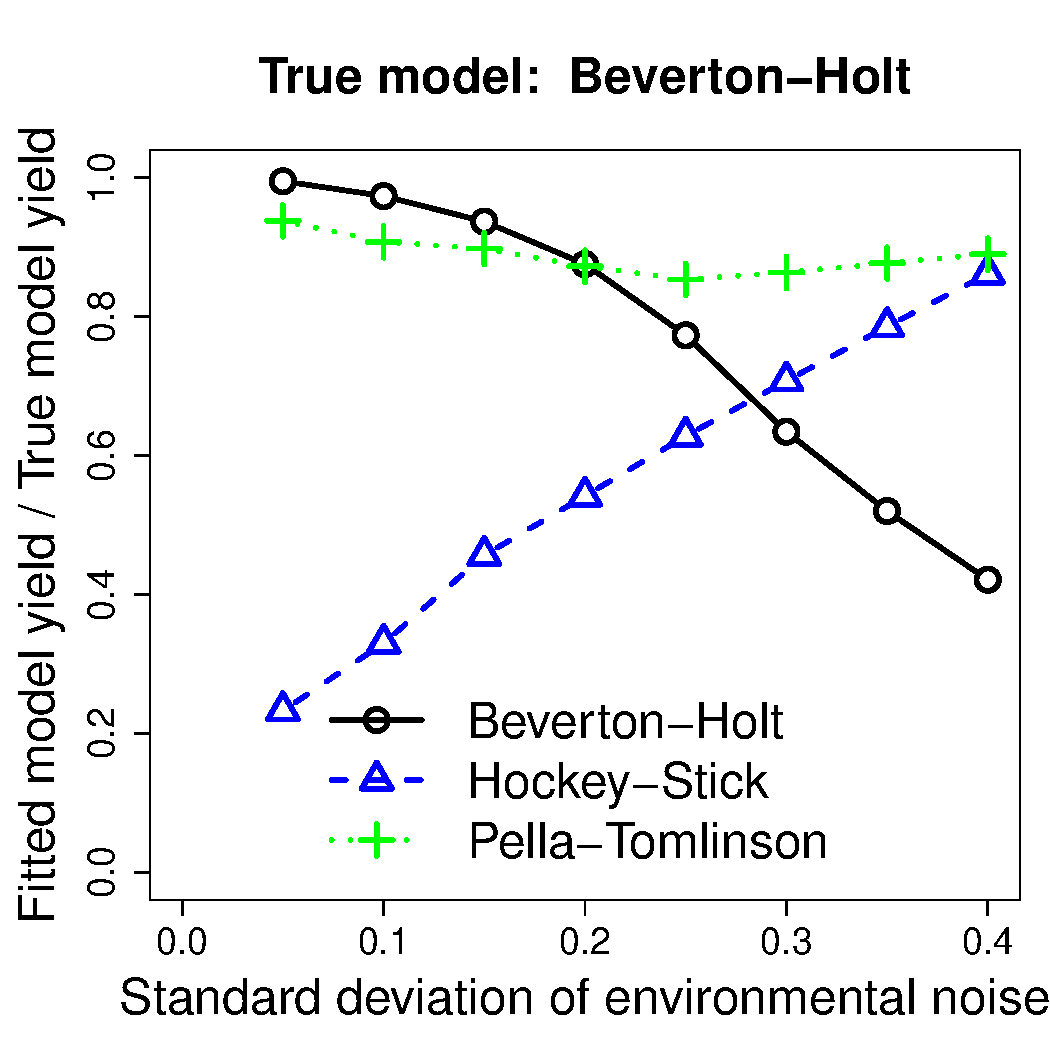
\includegraphics[width=\linewidth,valign=t]{True_1_relativeYield_sim.pdf}
	\end{subfigure}	
	\begin{subfigure}[t]{0.02\textwidth}
		\textbf{b)}
	\end{subfigure}
	\begin{subfigure}[t]{0.3\textwidth}
		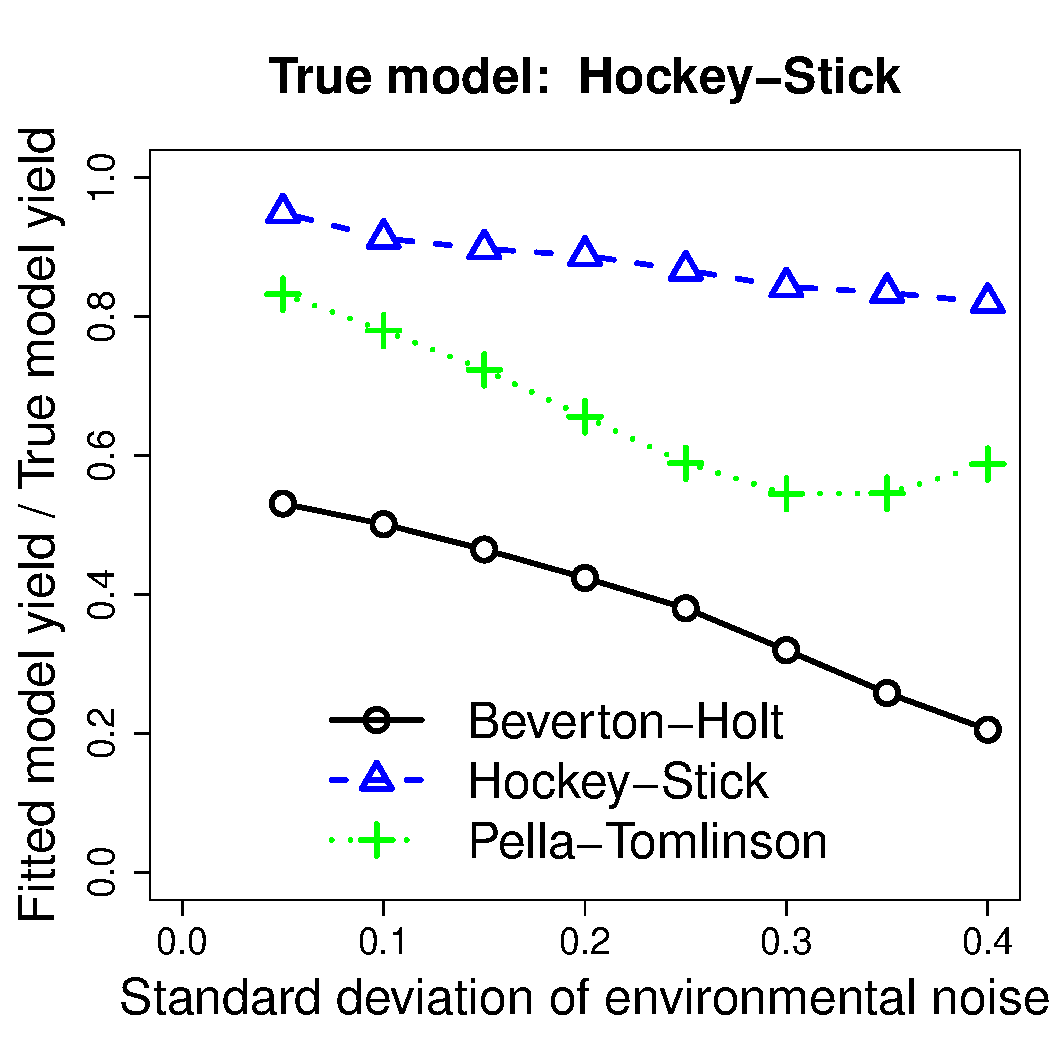
\includegraphics[width=\linewidth,valign=t]{True_2_relativeYield_sim.pdf}
	\end{subfigure}	
	\begin{subfigure}[t]{0.02\textwidth}
		\textbf{c)}
	\end{subfigure}
	\begin{subfigure}[t]{0.3\textwidth}
		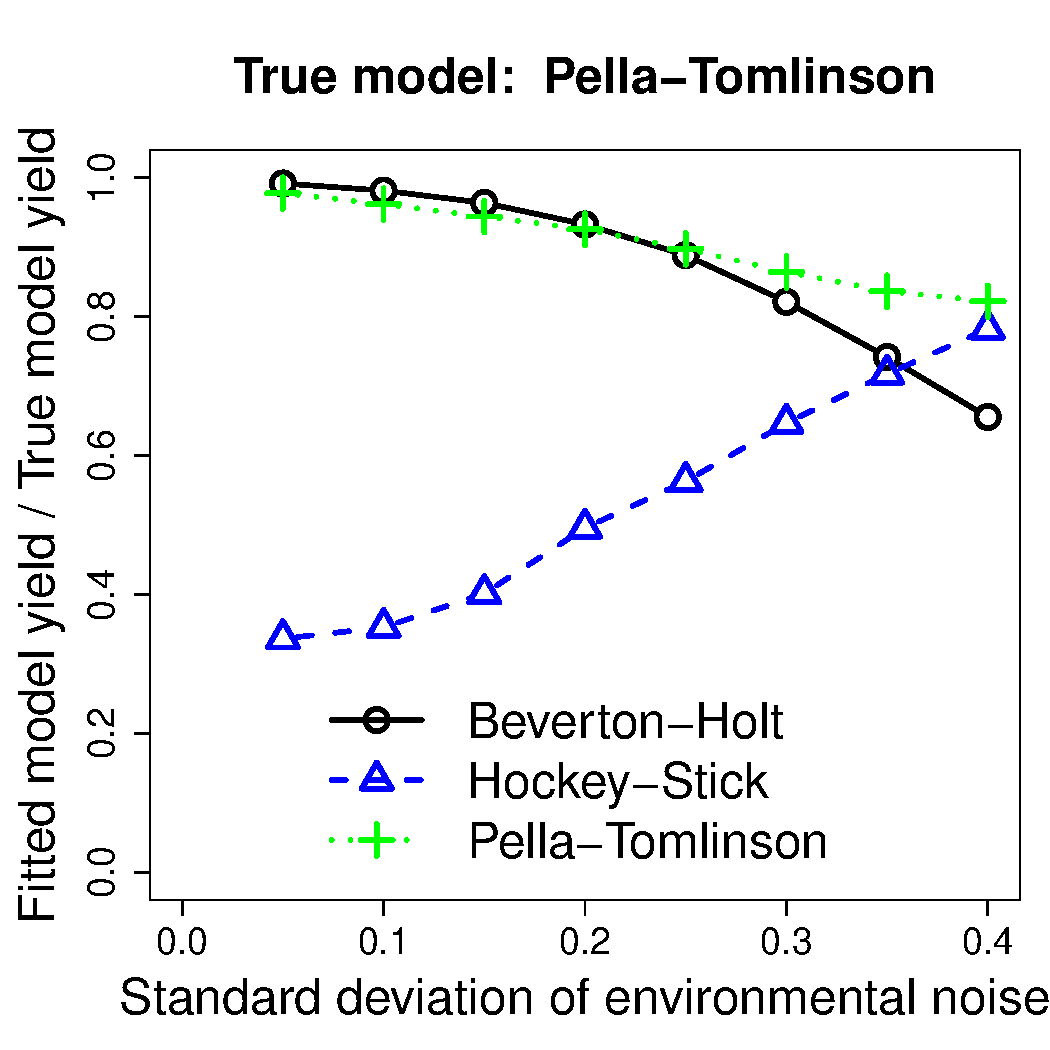
\includegraphics[width=\linewidth,valign=t]{True_3_relativeYield_sim.pdf}
	\end{subfigure}
	\begin{subfigure}[t]{0.02\textwidth}
		\textbf{d)}
	\end{subfigure}
	\begin{subfigure}[t]{0.3\textwidth}
		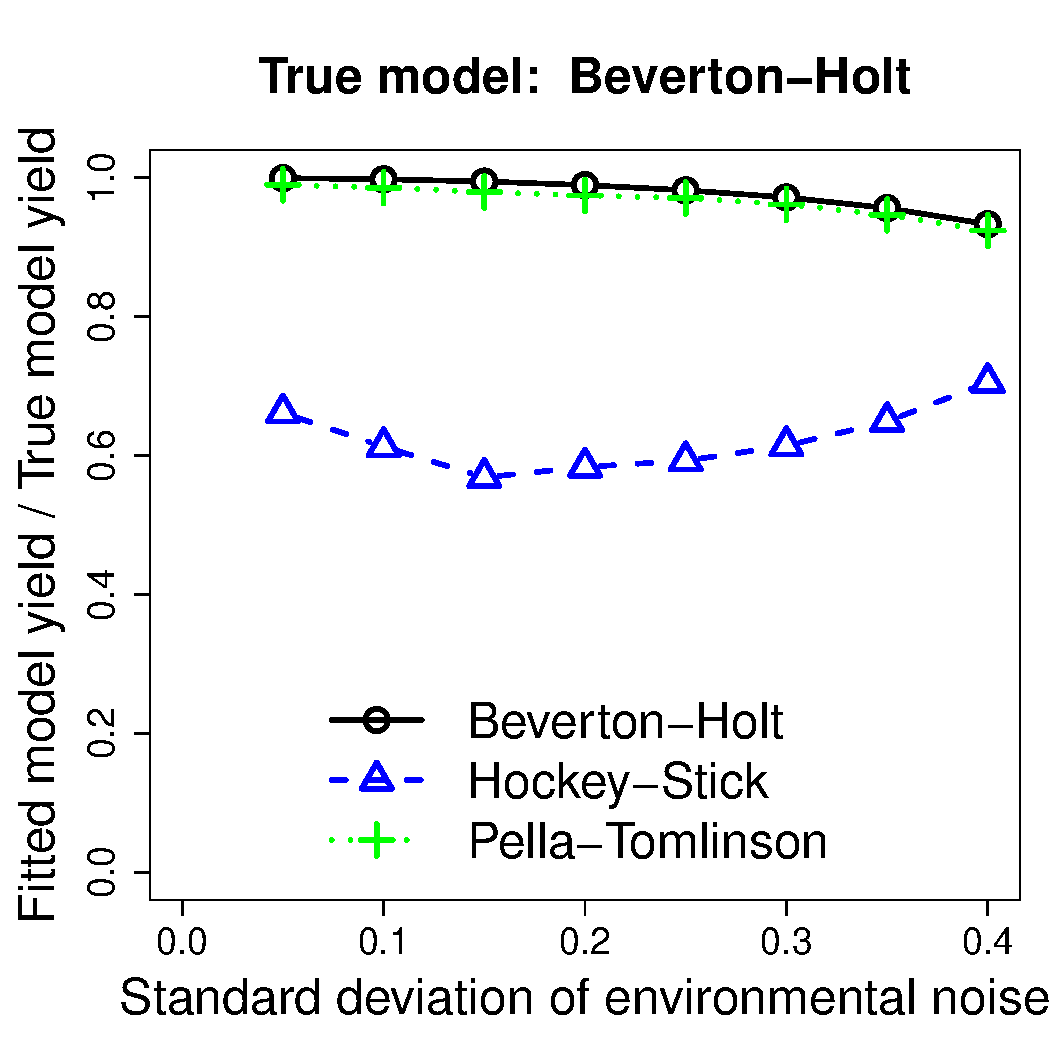
\includegraphics[width=\linewidth,valign=t]{True_1_relativeYield_sim_high_r.pdf}
	\end{subfigure}	
	\begin{subfigure}[t]{0.02\textwidth}
		\textbf{e)}
	\end{subfigure}
	\begin{subfigure}[t]{0.3\textwidth}
		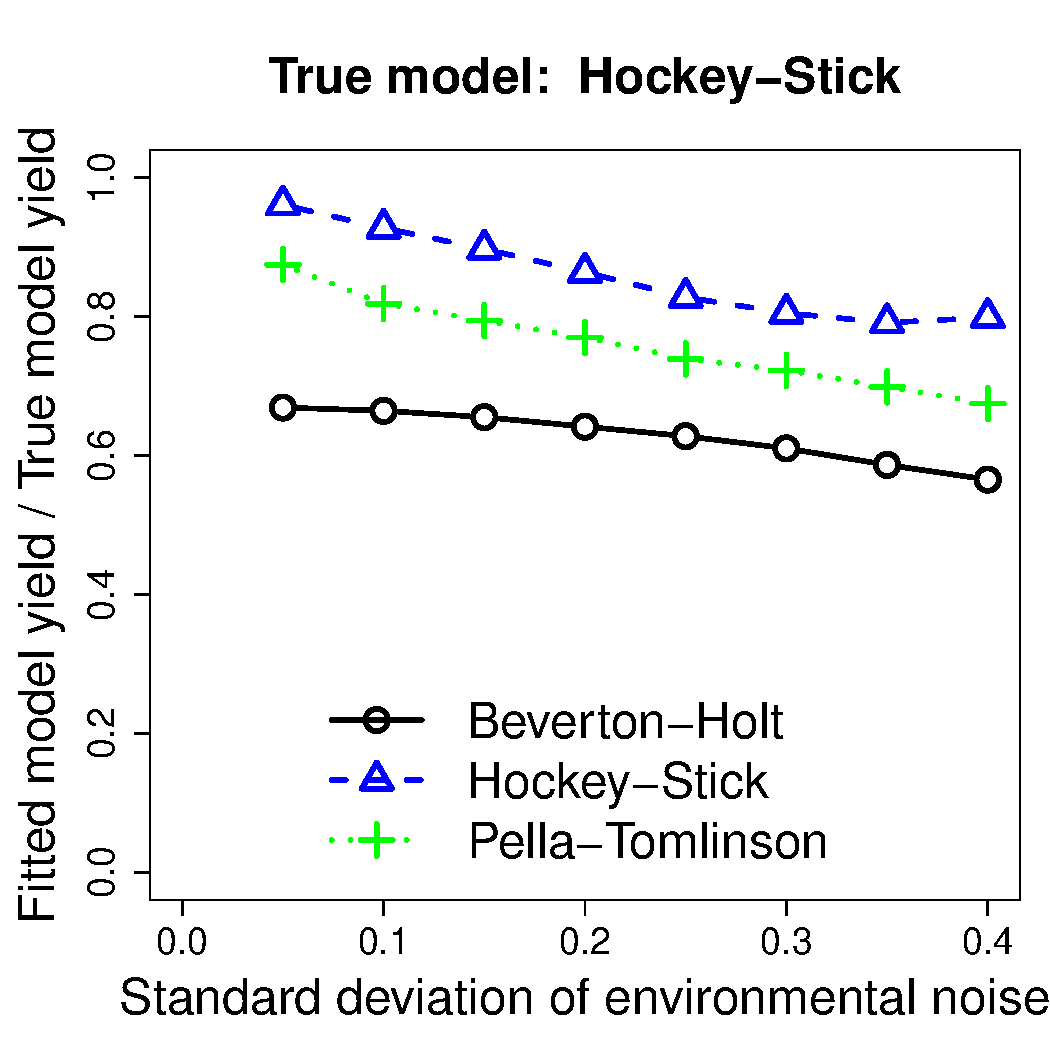
\includegraphics[width=\linewidth,valign=t]{True_2_relativeYield_sim_high_r.pdf}
	\end{subfigure}	
	\begin{subfigure}[t]{0.02\textwidth}
		\textbf{f)}
	\end{subfigure}
	\begin{subfigure}[t]{0.3\textwidth}
		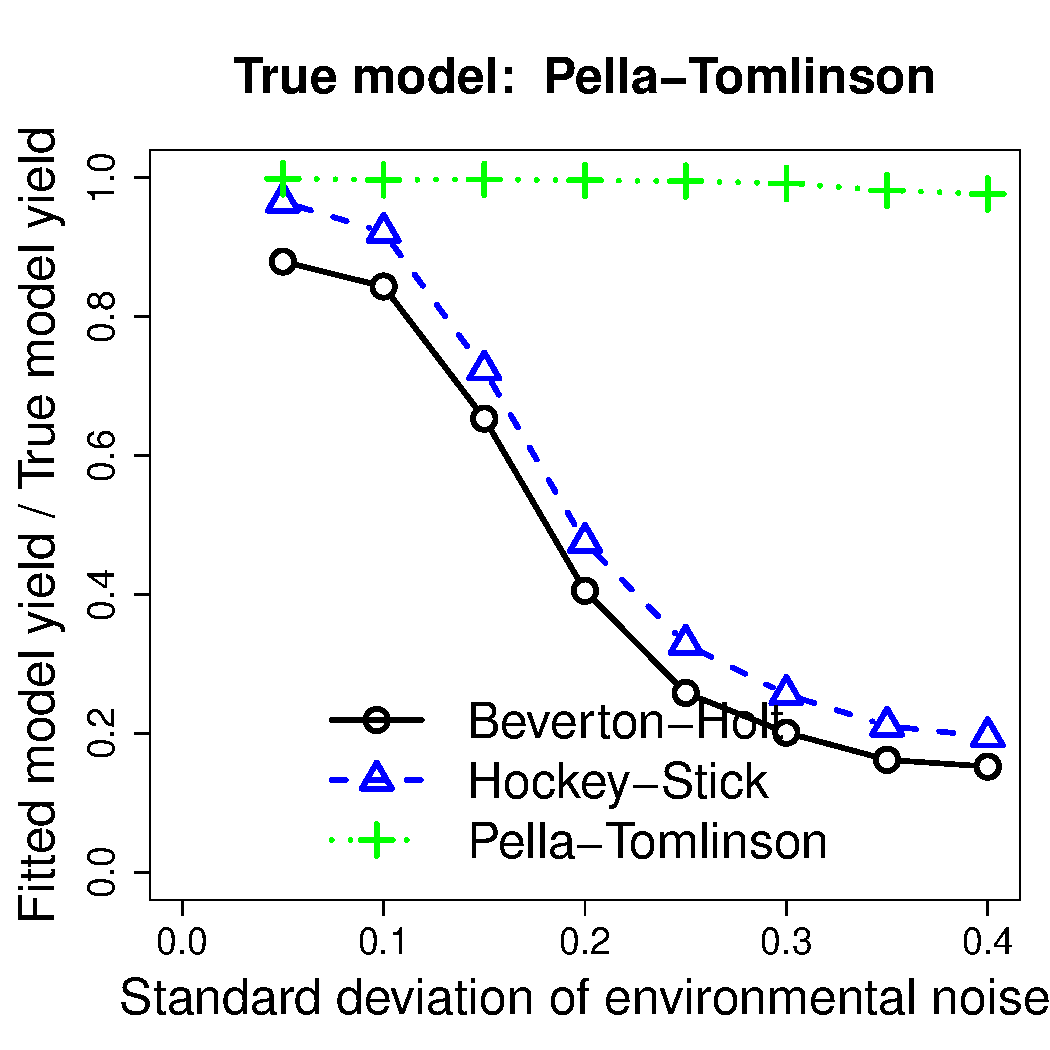
\includegraphics[width=\linewidth,valign=t]{True_3_relativeYield_sim_high_r.pdf}
	\end{subfigure}
	\caption{\textbf{Model Performance under alternative scenarios}. The curves are the means over $1,000$ simulations of harvest yield achieved using the optimal escapement rule produced by a fitted model (circle = Beverton-Holt, triangle = hockey-stick, cross = Pella-Tomlinson) divided by the corresponding yield achieved using the true optimal escapement rule with parameters known, for different values of the standard deviation of the environmental noise. In (row a-c) $r=0.15$, (row d-f) $r=1$. Each column is a different true model. In all plots, $k=100$, and for the Pella Tomlinson model $\phi = 1$.}\label{fig:ModelPerfVSig}
\end{figure}


\subsection{Southern Bluefin Tuna case-study}
We found that both the Beverton-Holt (SSE = 0.070) and Pella Tomlinson (SSE = 0.067) fit the southern bluefin tuna biomass and catch data from the RAM stock assessment database better than the Hockey-stick model (SSE = 0.088) (see Fig. \ref{fig:Tuna} for data and model fits). However, when simulating fish biomass from each of the three fitted blue fin tuna models, the Hockey-stick optimal escapement rule always did better than the other incorrect model (for example when the true model was Beverton Holt, the hockey stick escapement rule achieved 51\% of the yield generated using the Beverton Holt optimal escapement rule, and the Pella-Tomlinson rule only generated 27\% of optimal yield (see Table \ref{table:tuna}). The probability that the Hockey-stick model would do better than the other incorrect model, when the is generated by a Pella-Tomlinson or Beverton-Holt model, by random chance, is 1/9.


\begin{figure}[!htbp]
	\centering
	\begin{subfigure}[t]{0.02\textwidth}
		\textbf{a)}
	\end{subfigure}
	\begin{subfigure}[t]{0.3\textwidth}
		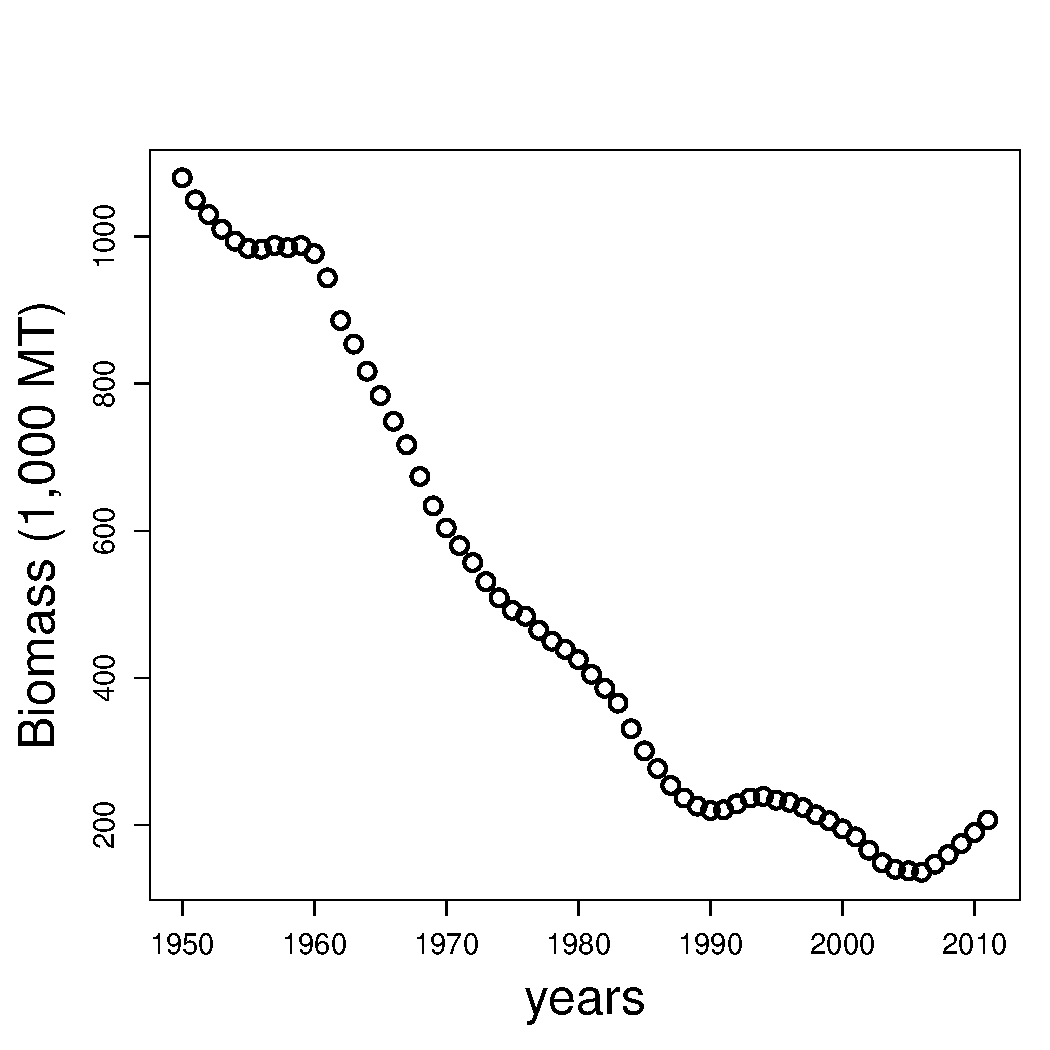
\includegraphics[width=\linewidth,valign=t]{TunaBiomass.pdf}
	\end{subfigure}	
	\begin{subfigure}[t]{0.02\textwidth}
		\textbf{b)}
	\end{subfigure}
	\begin{subfigure}[t]{0.3\textwidth}
		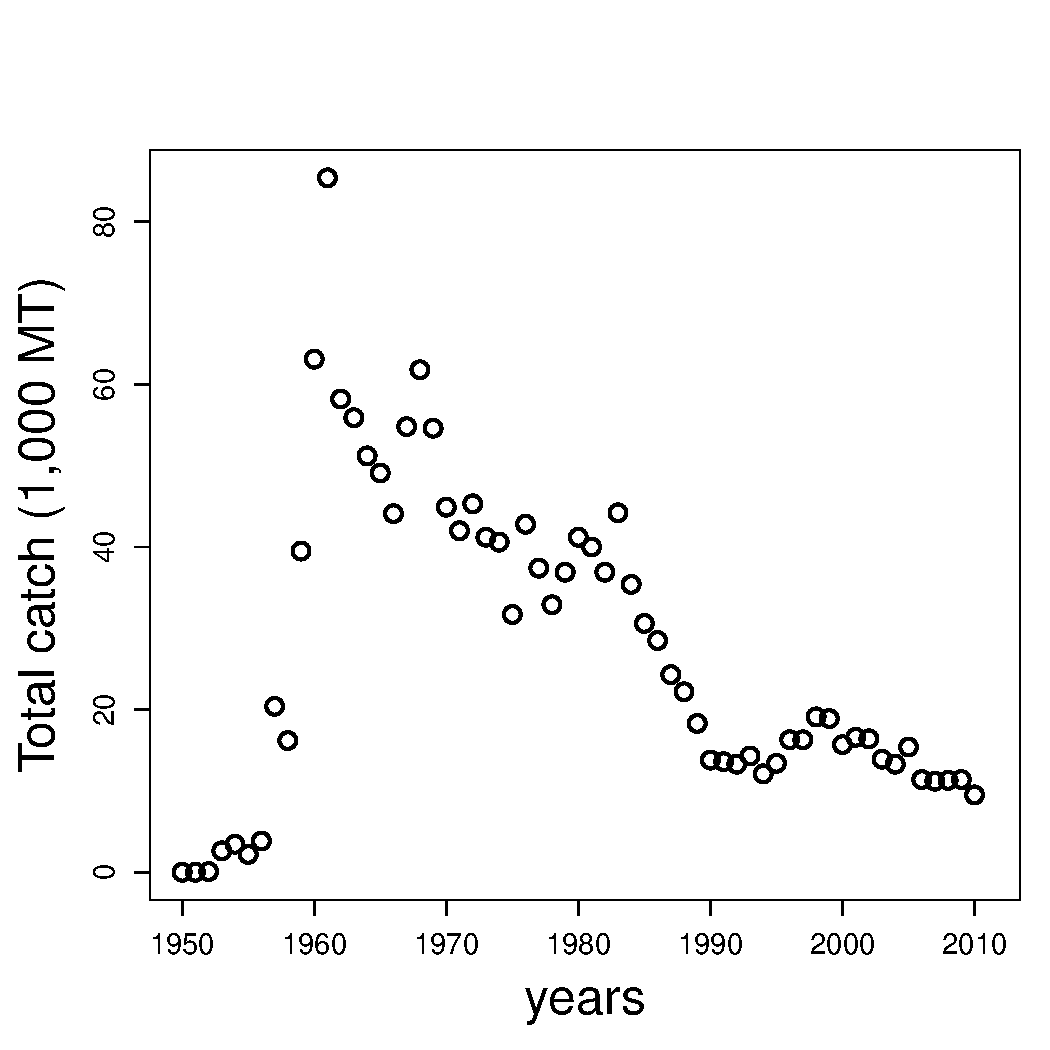
\includegraphics[width=\linewidth,valign=t]{TunaCatch.pdf}
	\end{subfigure}	
	\begin{subfigure}[t]{0.02\textwidth}
		\textbf{c)}
	\end{subfigure}
	\begin{subfigure}[t]{0.3\textwidth}
		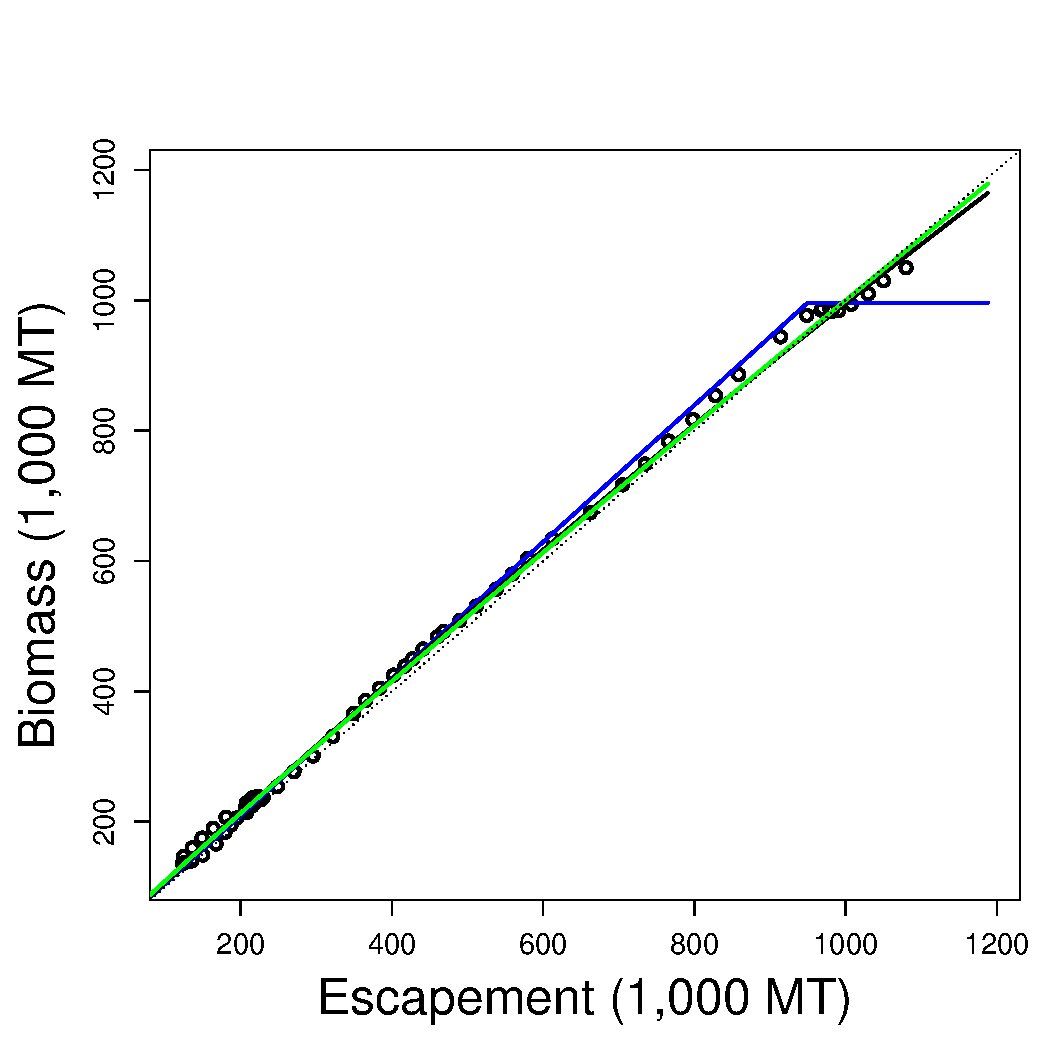
\includegraphics[width=\linewidth,valign=t]{FittedTuna.pdf}
	\end{subfigure}
	\caption{\textbf{Southern Bluefin tuna} (a) biomass and (b) catch time series data in thousands of metric tons. (c) Fitted Beverton-Holt (black), Hockey-stick (blue) and Pella Tomlinson (green) production functions to the data. Escapement is the biomass that escapes harvest in year $t$, $B_t - h_t$, and biomass is the resulting biomass in year $t+1$, $B_{t+1}$.}\label{fig:Tuna}
\end{figure}

\begin{table}[!htbp]
	\setlength{\extrarowheight}{2pt}
	\begin{tabular}{cc|c|c|c|}
		& \multicolumn{1}{c}{} & \multicolumn{3}{c}{Manager's Model} \\
		& \multicolumn{1}{c}{} & \multicolumn{1}{c}{$BH$}  & \multicolumn{1}{c}{$HS$}  & \multicolumn{1}{c}{$PT$} \\\cline{3-5}
		& $BH$ & $1$ & $0.513$ & $0.271$ \\ \cline{3-5}
		Assumed True Model  & $HS$ & $0.487$ & $1$ & $0.071$ \\\cline{3-5}
		& $PT$ & $0.410$ & $0.840$ & $1$ \\\cline{3-5}
	\end{tabular}
	\caption{Relative performance of optimal escapement strategies, generated by fitting Beverton-Holt (BH), Hockey-Stick (HS), and Pella-Tomlinson (PT) models (columns) to time series data on Southern Bluefin Tuna, in comparison to the true model as in the rows. Each column denotes the perormance of the model. The hockey-stick model performces best compared to all other incorrect models.}\label{table:tuna}
\end{table}

\section{Discussion / potential directions to take this paper}

\begin{itemize}
	\item Caveat: correlations between $r$, $k$ and $\phi$ can lead to poor model fits (literature on theta logistic models \citep{polansky2009,clark2010theta} ). It is also unclear to me why the $(\theta + 1)/\theta$ scaling is used in some works and not in others, it might be a statistical fitting issue.
	\item Caveat: If we instead of looking at column sums from  table \ref{table:tuna} (which assumes uniform uncertainty among the models), we look at weighted column sums by something like a relative AIC, do the results change? For example Hockey-Stick does the best when false, but it is also the most liekly to be false (i.e. has the worst model fit to the data).
	\item Direction: If we repeat table \ref{table:tuna} for several species in RAM would we find a pattern. Perhaps slow growing fish tend to be best managed via a hockeystick model?
	\item Future direction: what happens when the "true model" is a randomly generated lotka-voltera style food-web and we do stock assessment using these single species models. Do certain single species production functions do best at managing a fish within the greater context of an ecosystem (probably a seperate paper).
\end{itemize}          
          
\section*{References}\label{references}
\bibliography{NearKEscapement}

\addcontentsline{toc}{section}{References}

\hypertarget{refs}{}

\end{document}


